\appendix
\addcontentsline{toc}{section}{Appendices}
\renewcommand{\thesection}{\Alph{section}}

\section{Statement on Generative AI Usage}
In the preparation and execution of this capstone project, I employed generative artificial intelligence (AI) tools—including OpenAI's ChatGPT, Anthropic's Claude AI, and Perplexity.ai—as performance-enhancing resources. These tools were used responsibly and transparently in accordance with ethical research and academic integrity guidelines.

Specifically, generative AI assisted in the following ways:
\begin{itemize}
    \item \textbf{Proofreading and Editing:} Refining academic tone, grammar, and clarity in LaTeX narrative sections and technical documentation.
    \item \textbf{Code Development and Debugging:} Supporting complex problem-solving in Python (e.g., data analysis, visualization, and machine learning workflows) and LaTeX (e.g., formatting, cross-referencing, and table construction).
    \item \textbf{Learning Support:} Providing explanations, examples, and clarifications that supplemented my independent understanding of technical subjects such as CRISP-DM methodology, geospatial visualization, and clustering algorithms.
\end{itemize}

All analytical design, data interpretation, modeling decisions, and final editorial control were my own. The use of AI was strictly as a learning augmentation and productivity aid, not a replacement for critical thinking, domain expertise, or original work. I acknowledge these tools as part of a modern, evolving data science workflow that demands both technical proficiency and ethical responsibility.


\section{Regional Overview of North Central Arkansas}

\begin{table}[H]
\centering
\caption{North Central Arkansas (NCA) Counties}
\label{tab:appendix_nca_counties}
\begin{tabular}{ll}
\toprule
\textbf{County Name} & \textbf{Notes} \\
\midrule
Baxter         & Core Ozark Highlands \\
Boone          & Adjacent to Missouri border \\
Fulton         & Northeastern NCA \\
Izard          & Central education corridor \\
Marion         & Buffalo National River access \\
Newton         & Sparsely populated Ozark terrain \\
Searcy         & High-risk outlier regionally \\
Sharp          & Includes Highland, Cherokee Village \\
Stone          & Cultural hub (e.g., Mountain View) \\
Van Buren      & Ozark-River Valley border \\
Cleburne       & Greers Ferry Lake area \\
Independence   & Batesville, economic anchor \\
Lawrence       & Northeastern fringe of NCA \\
\bottomrule
\end{tabular}
\end{table}

\section{CRISP-DM Framework Guide}
The Cross-Industry Standard Process for Data Mining (CRISP-DM) is a robust, domain-agnostic methodology that guides the development and execution of data science projects. Originally developed to formalize best practices in industrial data mining, it has since been widely adopted across sectors including business, education, healthcare, and government. CRISP-DM divides the analytic process into six iterative phases, promoting a structured yet flexible workflow that emphasizes interpretability, stakeholder alignment, and reproducibility.

\begin{enumerate}
    \item \textbf{Business Understanding} \\
    This initial phase defines the project’s objectives from a stakeholder perspective. It involves translating broad goals into specific, data-oriented questions. A deep understanding of the domain—whether it is finance, public health, education, or manufacturing—is critical to framing relevant problems, determining project scope, and identifying potential constraints or success criteria.

    \item \textbf{Data Collection (Data Understanding)} \\
    The second phase focuses on acquiring relevant data and developing familiarity with its structure and limitations. Tasks include identifying appropriate data sources, understanding formats and metadata, assessing data quality, and performing preliminary explorations. This phase often reveals inconsistencies, missing values, or unexpected distributions that can influence future modeling decisions.

    \item \textbf{Data Preparation} \\
    Often the most time-intensive step, data preparation involves transforming raw data into a structured format suitable for analysis. This includes cleaning (handling missing values, correcting errors), integrating multiple datasets, engineering new features, and standardizing variables. The quality of this phase directly impacts the effectiveness of modeling and interpretation.

    \item \textbf{Modeling} \\
    In this phase, statistical or machine learning models are selected and applied to address the core research questions. Techniques vary depending on the objective—classification, clustering, regression, anomaly detection, etc.—and model performance is influenced by both algorithm choice and data structure. Model building is iterative, often requiring adjustments based on evaluation outcomes.

    \item \textbf{Evaluation} \\
    Once models are built, their outputs must be assessed for validity, accuracy, and relevance. Evaluation includes both quantitative measures (e.g., accuracy, RMSE, silhouette score) and qualitative judgment (e.g., interpretability, alignment with domain expectations). A model that performs well statistically but fails to provide actionable insight may require refinement or replacement.

    \item \textbf{Deployment} \\
    The final phase delivers the results in a format that supports decision-making. This may involve generating reports, dashboards, presentations, or embedding models into production environments. Successful deployment also includes documenting methodology, limitations, and recommendations, ensuring transparency and future adaptability.

\end{enumerate}

\noindent The CRISP-DM model is not strictly linear. Practitioners frequently cycle back to earlier phases as new insights emerge, making it an inherently iterative process. Its emphasis on clarity, flexibility, and domain alignment makes it particularly effective for interdisciplinary applications of data science.

\noindent For more detailed information, visit: \\
\href{https://www.datascience-pm.com/crisp-dm-2/}{https://www.datascience-pm.com/crisp-dm-2/}


\section{Project Structure}
\begin{figure}[H]
\centering
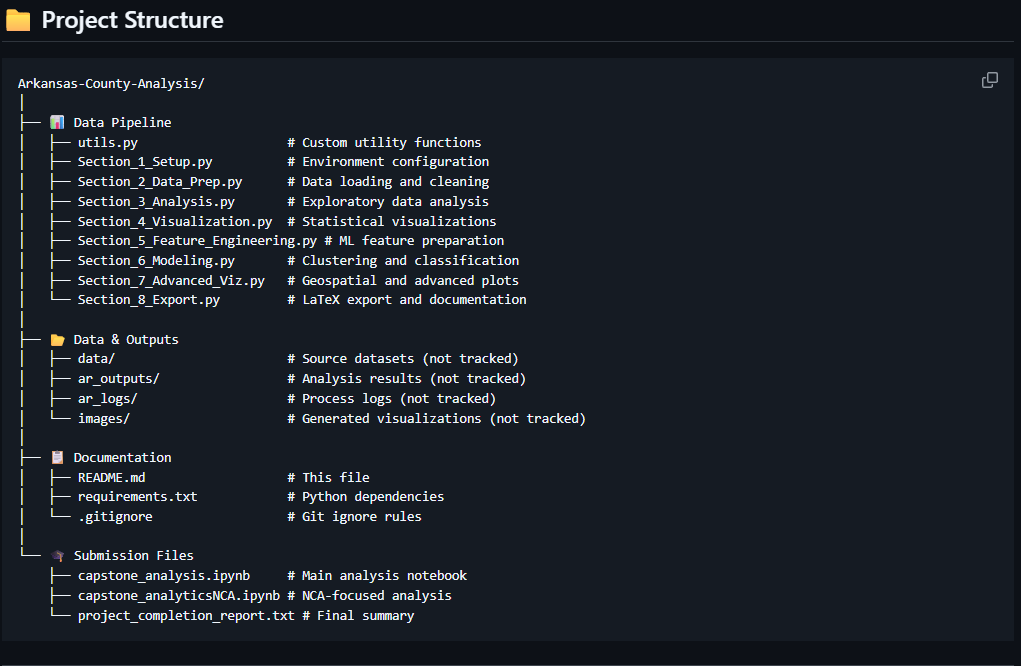
\includegraphics[width=0.95\textwidth]{proj_structure.png}
\caption{Project Structure: End-to-end analytic pipeline used in this project, following the CRISP-DM framework.}
\label{fig:project_diagram}
\end{figure}


\section{Full-Scale Bivariate Visualizations}
This appendix presents full-scale versions of the four bivariate visualizations. These graphics compare county-level metrics across Arkansas, with particular attention to counties in North Central Arkansas (NCA), which are visually highlighted for regional comparison.

\begin{figure}[H]
\centering
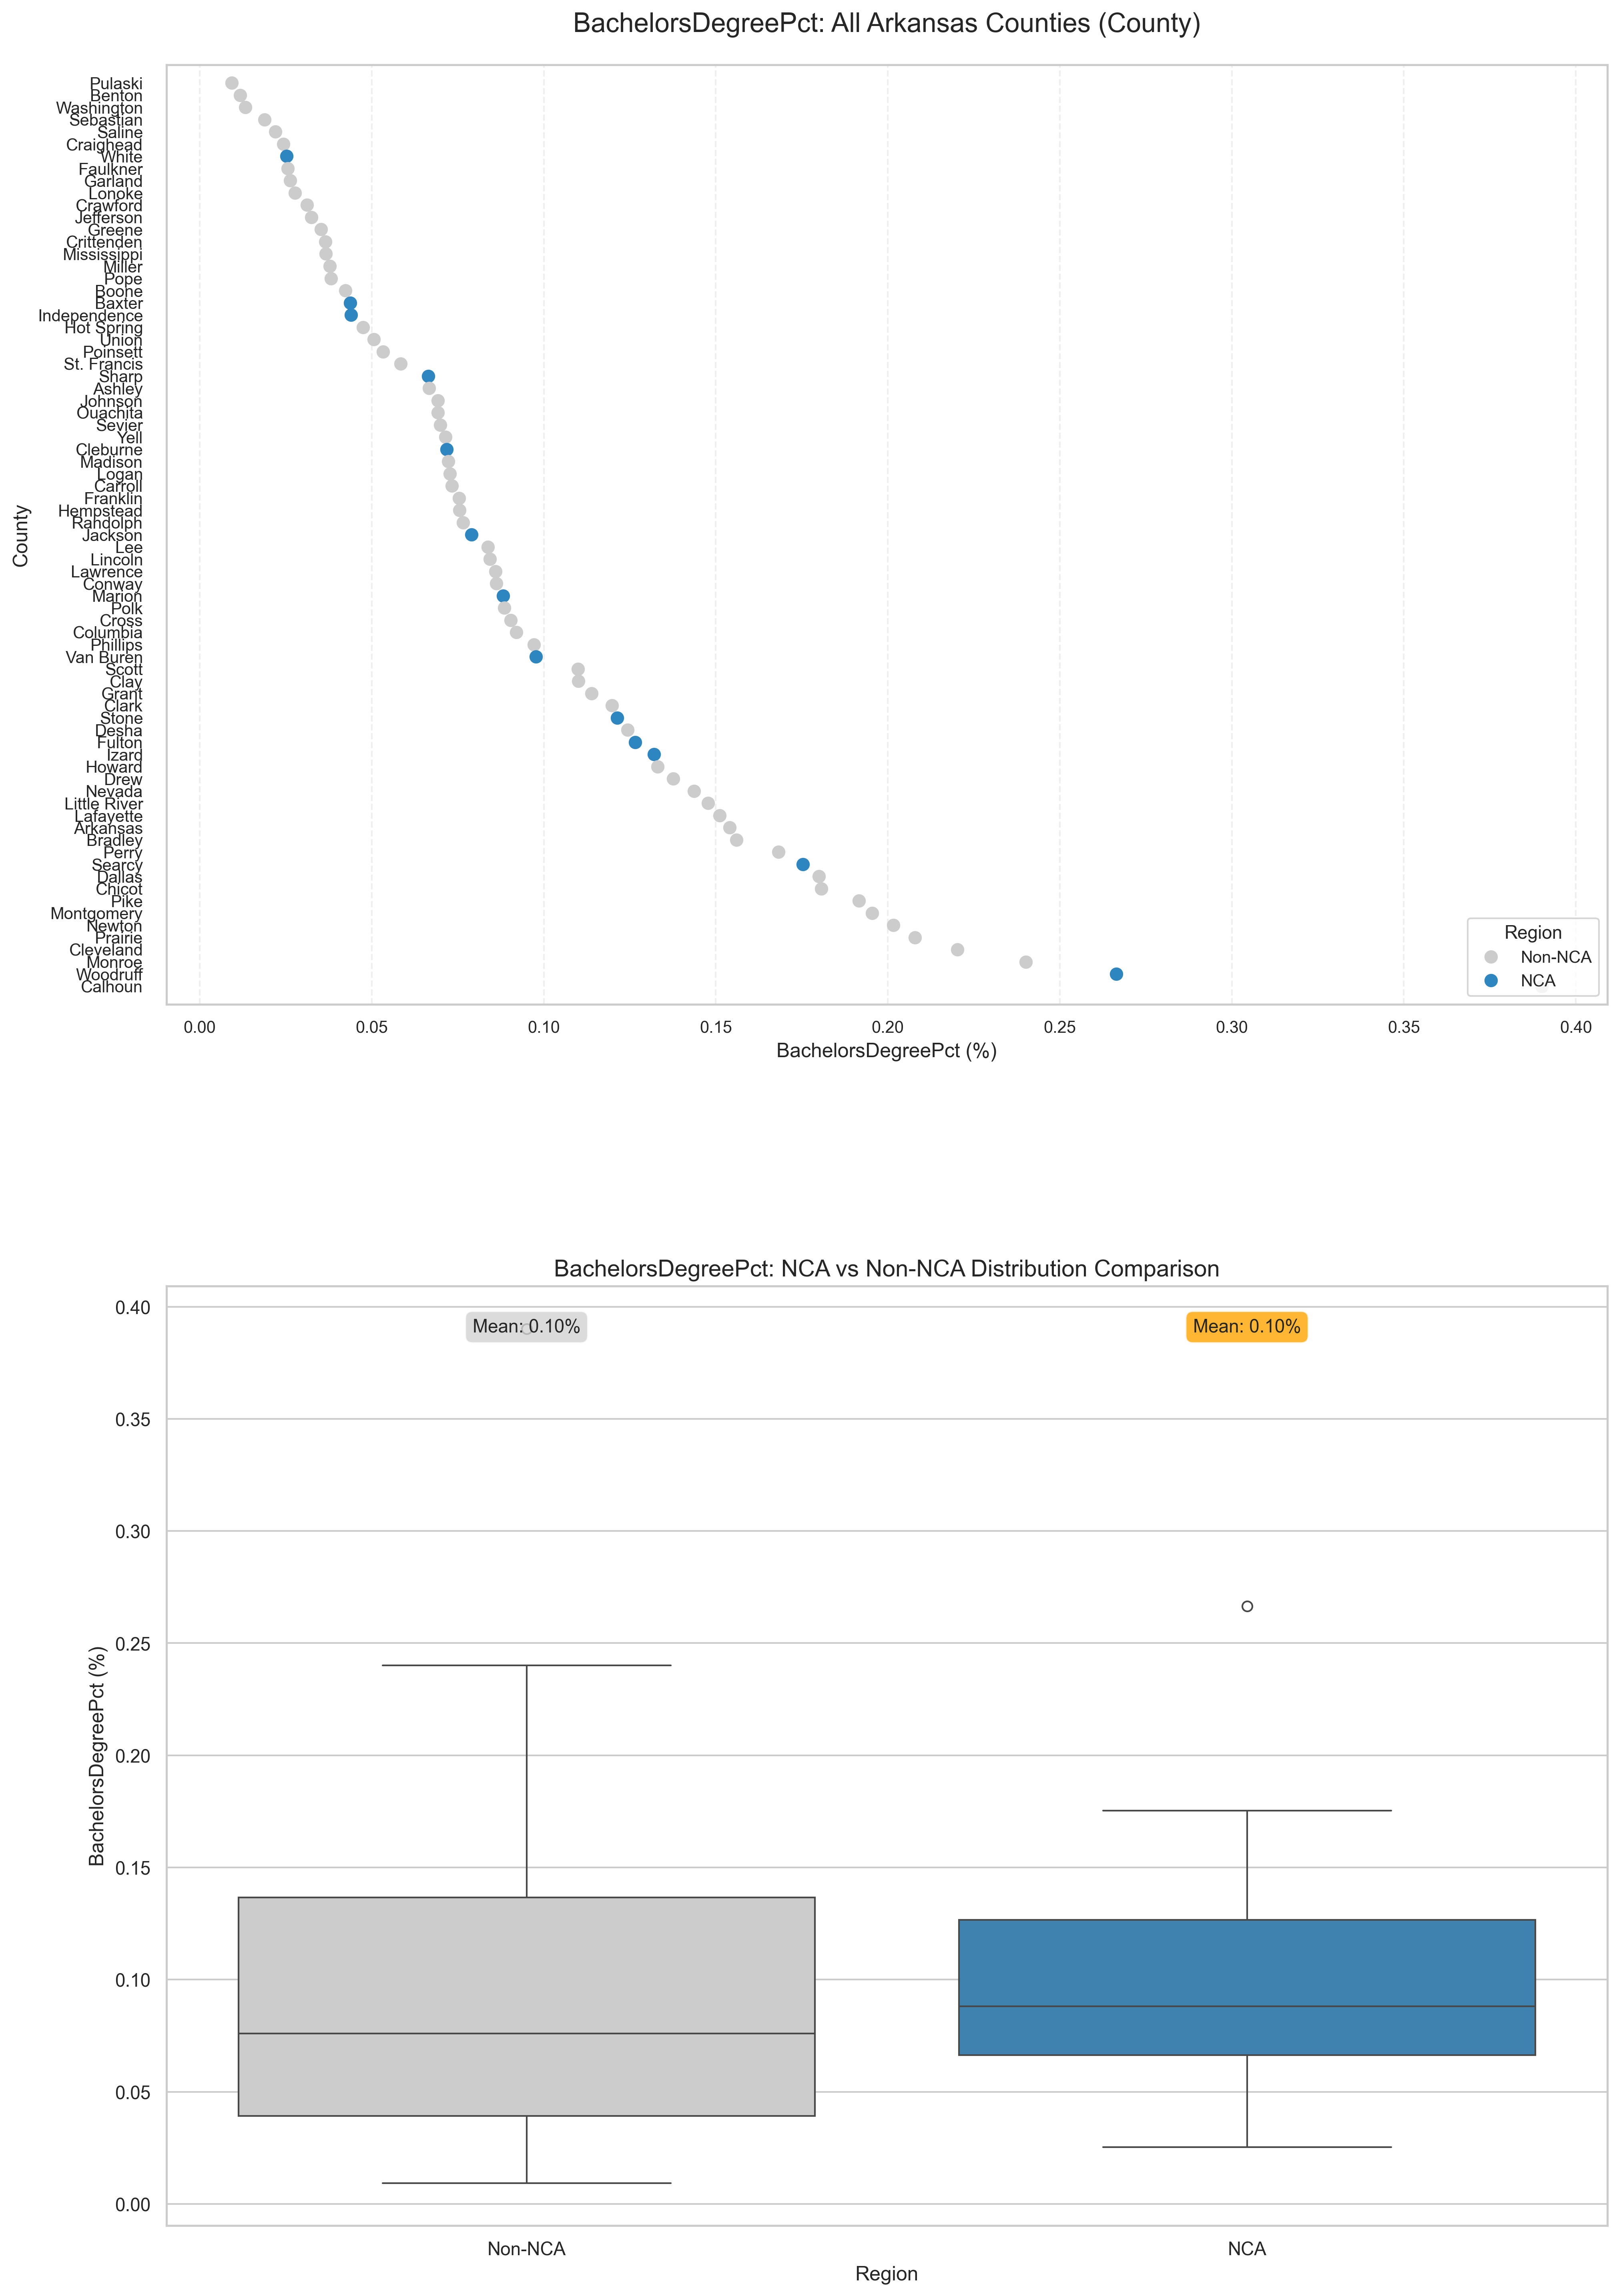
\includegraphics[width=0.95\textwidth]{Capstone_Project_Report/images/maps/nca_comparison_bachelorsdegreepct.png}
\caption{Bivariate Comparison of Educational Attainment: This figure highlights bachelor’s degree attainment across all Arkansas counties, with NCA counties marked distinctly. The visual emphasizes the persistent educational attainment gap faced by rural regions such as North Central Arkansas, where the proportion of residents with bachelor’s degrees tends to fall well below the state average.}
\label{fig:appendix_bachelors}
\end{figure}

\begin{figure}[H]
\centering
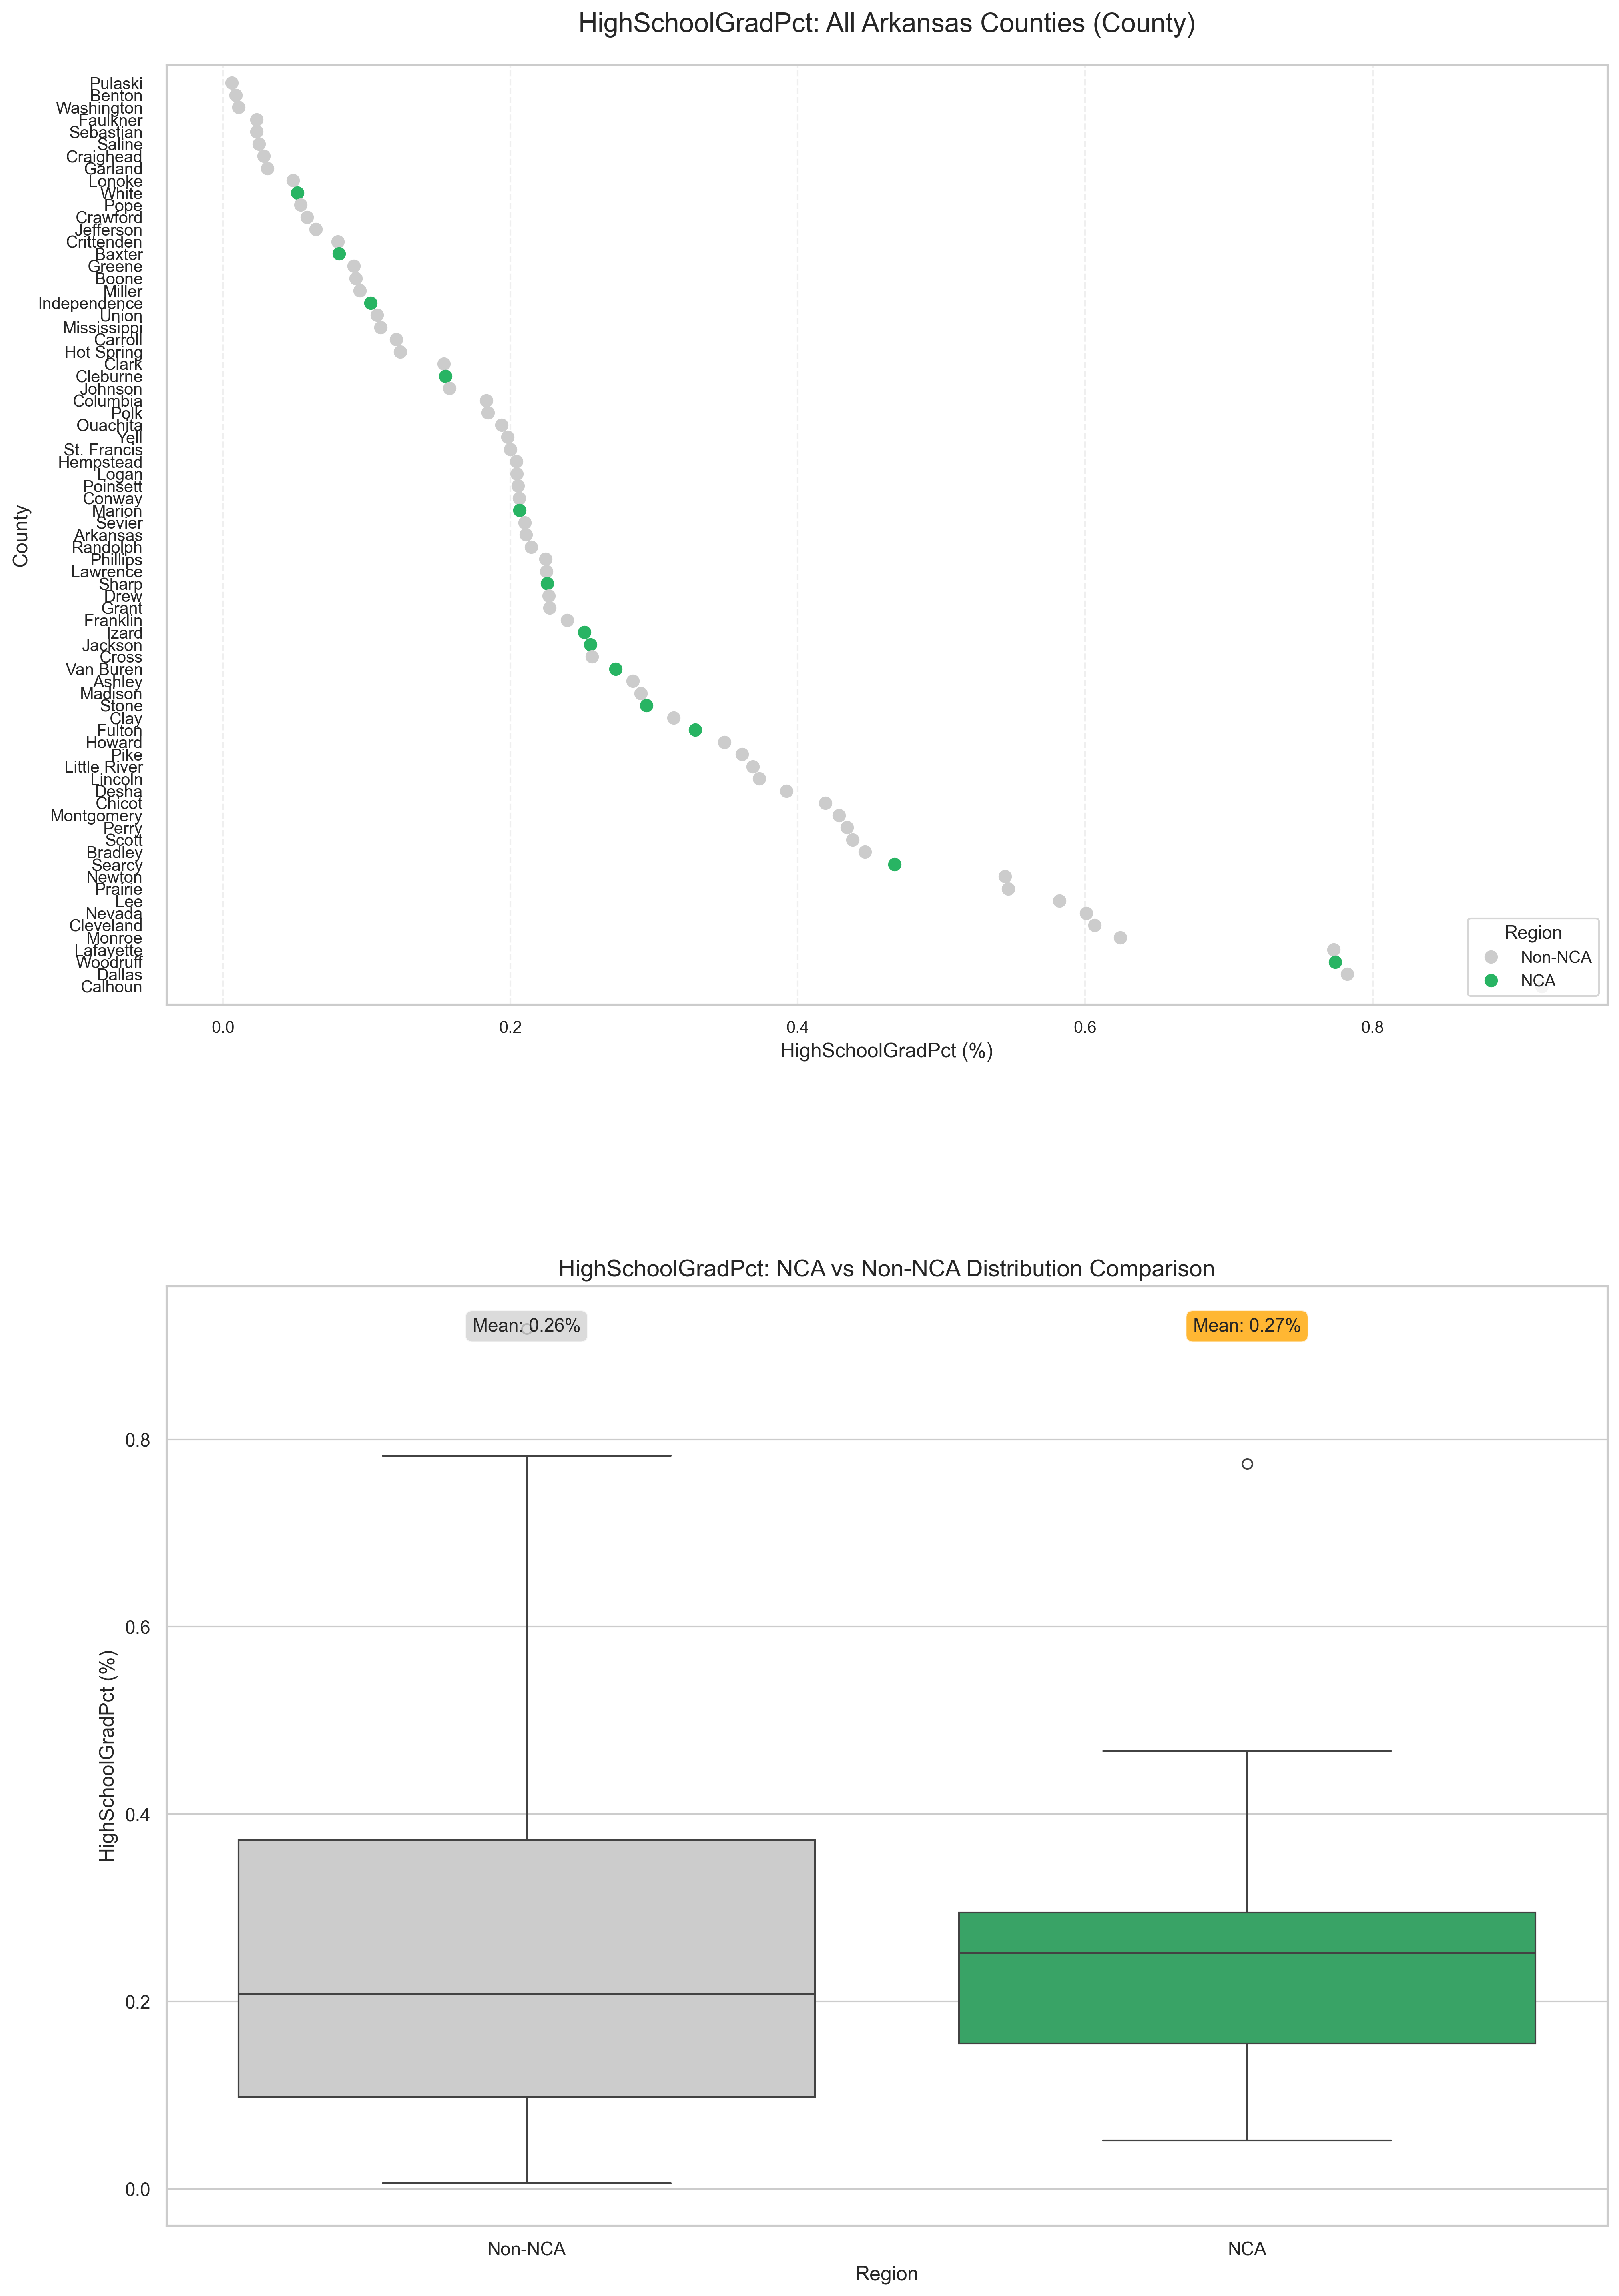
\includegraphics[width=0.95\textwidth]{Capstone_Project_Report/images/maps/images_nca_comparison_highschoolgradpct.png}
\caption{Bivariate Comparison of High School Graduation Rates: Graduation percentages in NCA counties (in green) are mixed, with most falling slightly below the statewide norm..}
\label{fig:appendix_vulnerability}
\end{figure}

\begin{figure}[H]
\centering
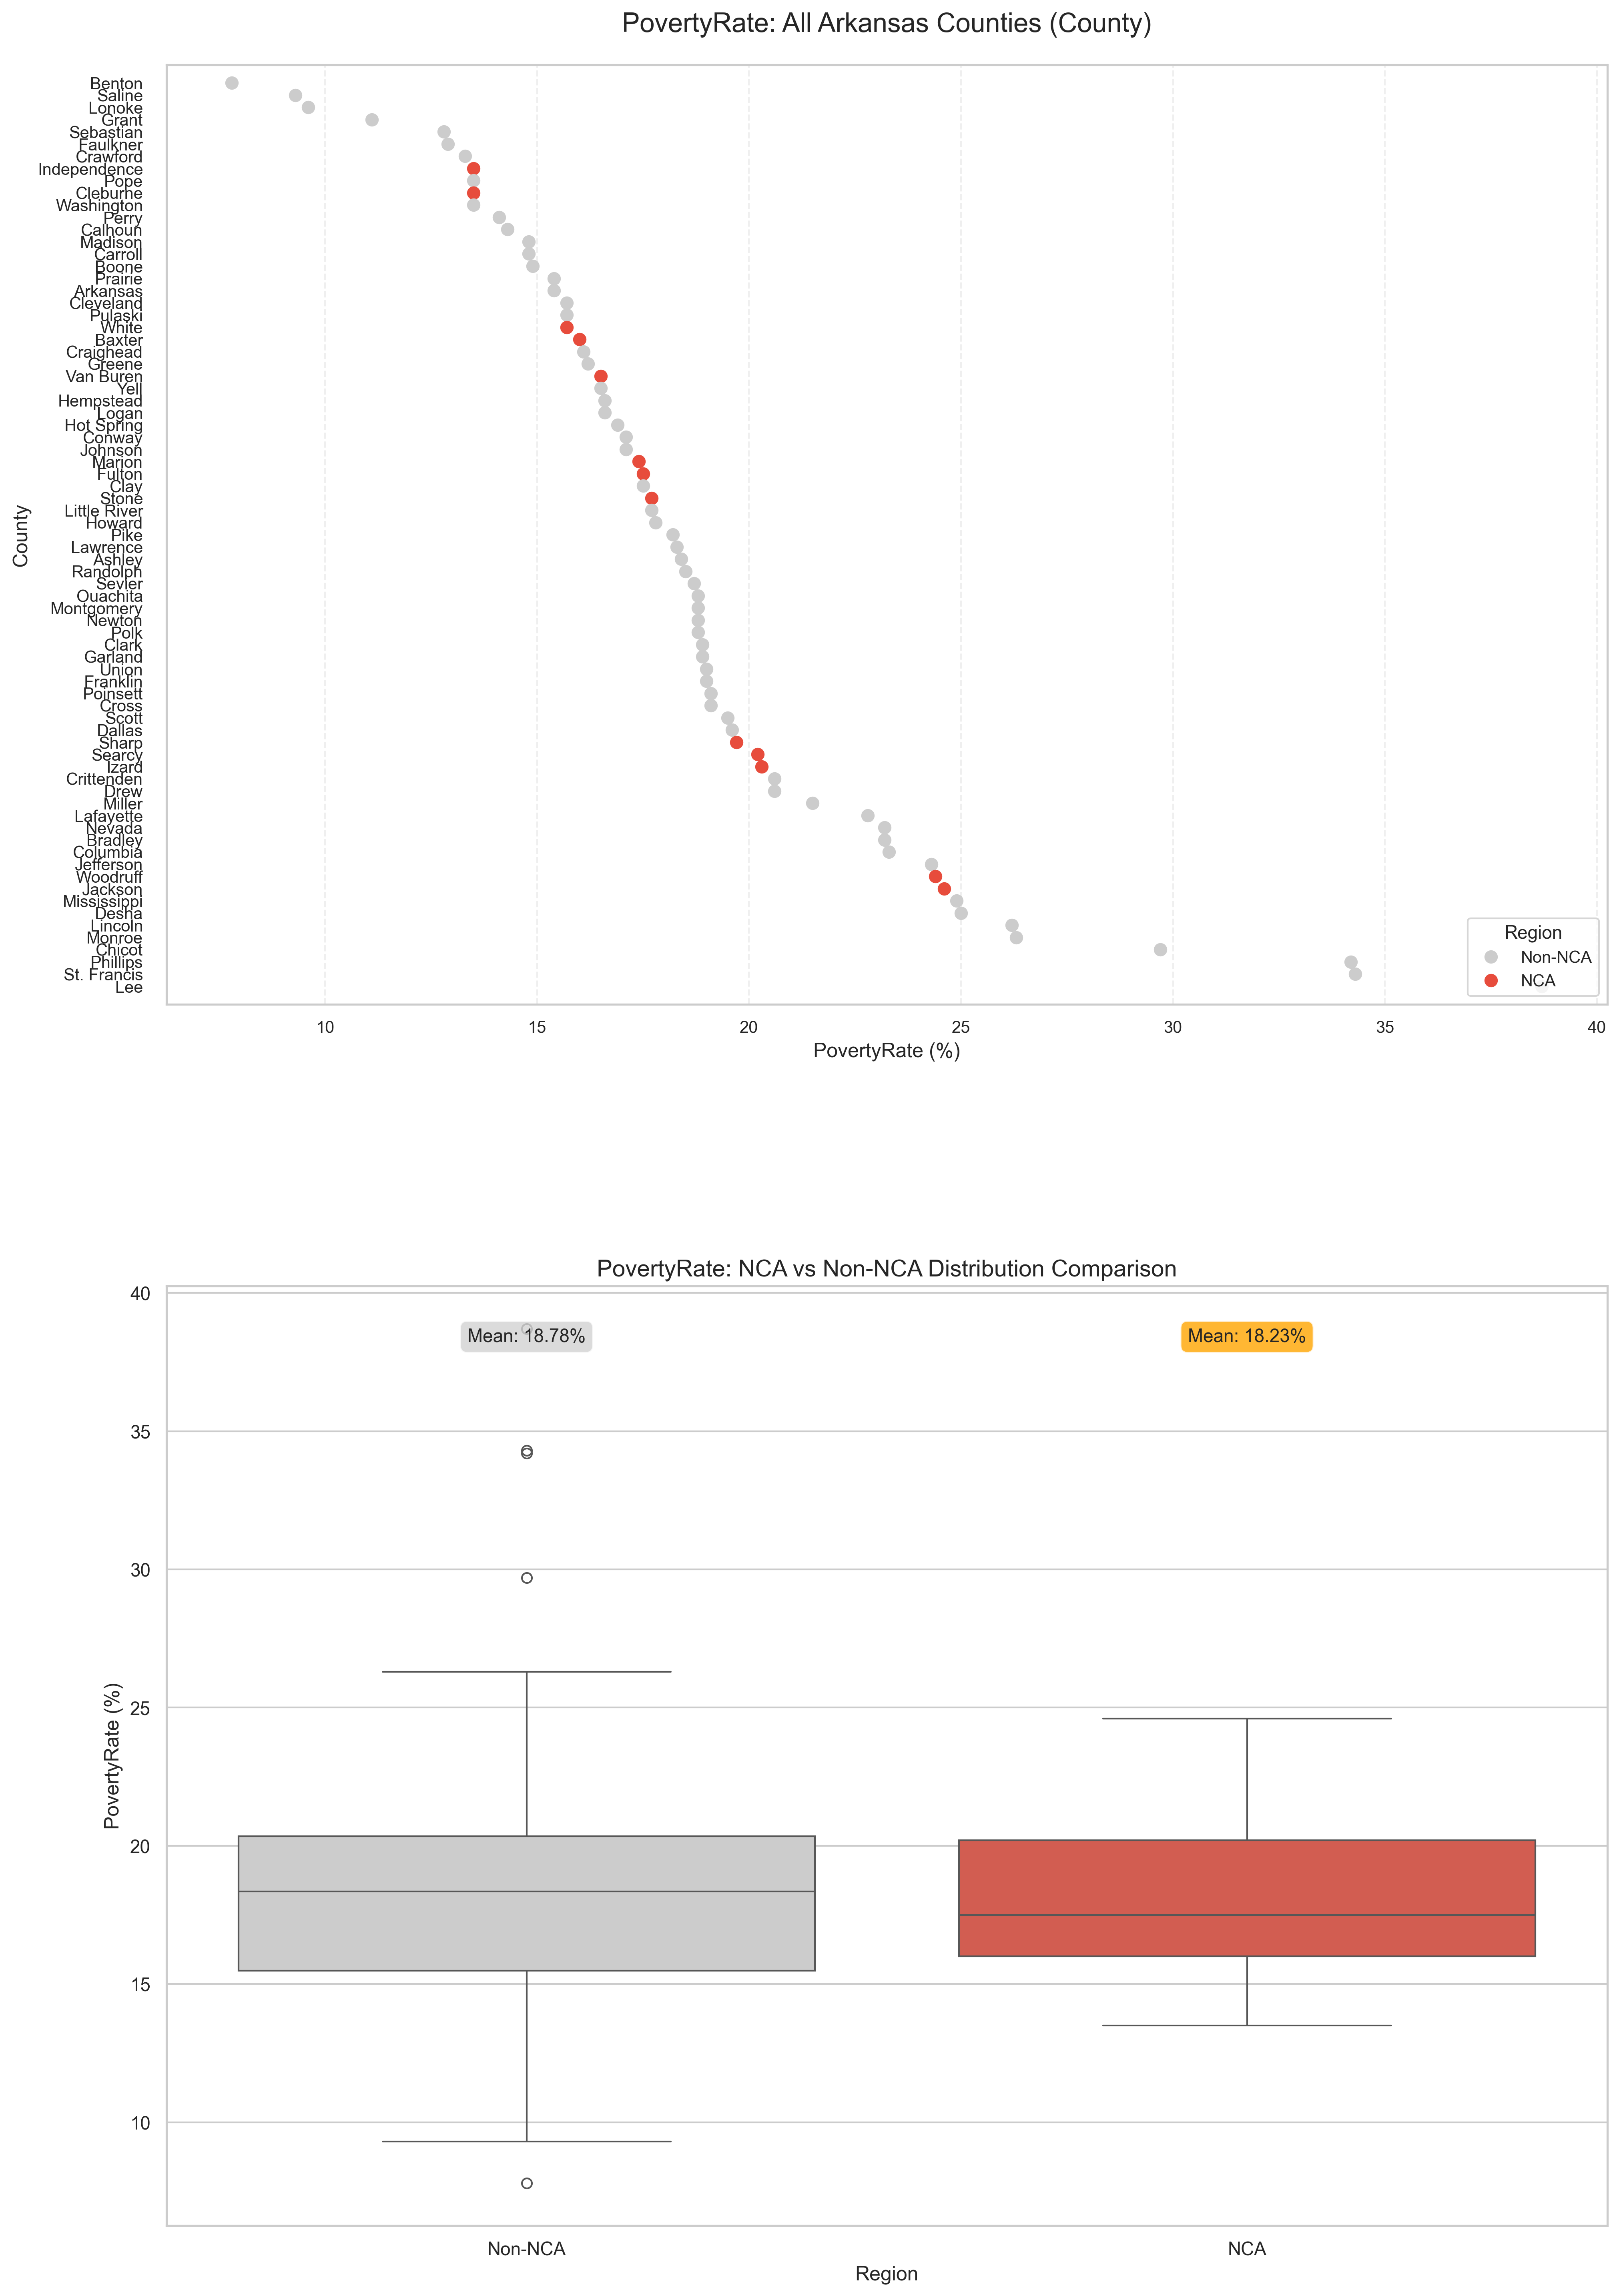
\includegraphics[width=0.95\textwidth]{Capstone_Project_Report/images/maps/nca_comparison_povertyrate.png}
\caption{Bivariate Comparison of Poverty Rates: Several counties in North Central Arkansas appear above the trendline for poverty, suggesting elevated economic burden relative to similarly structured counties. This visualization reinforces the relationship between limited educational access and persistent poverty within the region.}
\label{fig:appendix_poverty}
\end{figure}

\begin{figure}[H]
\centering
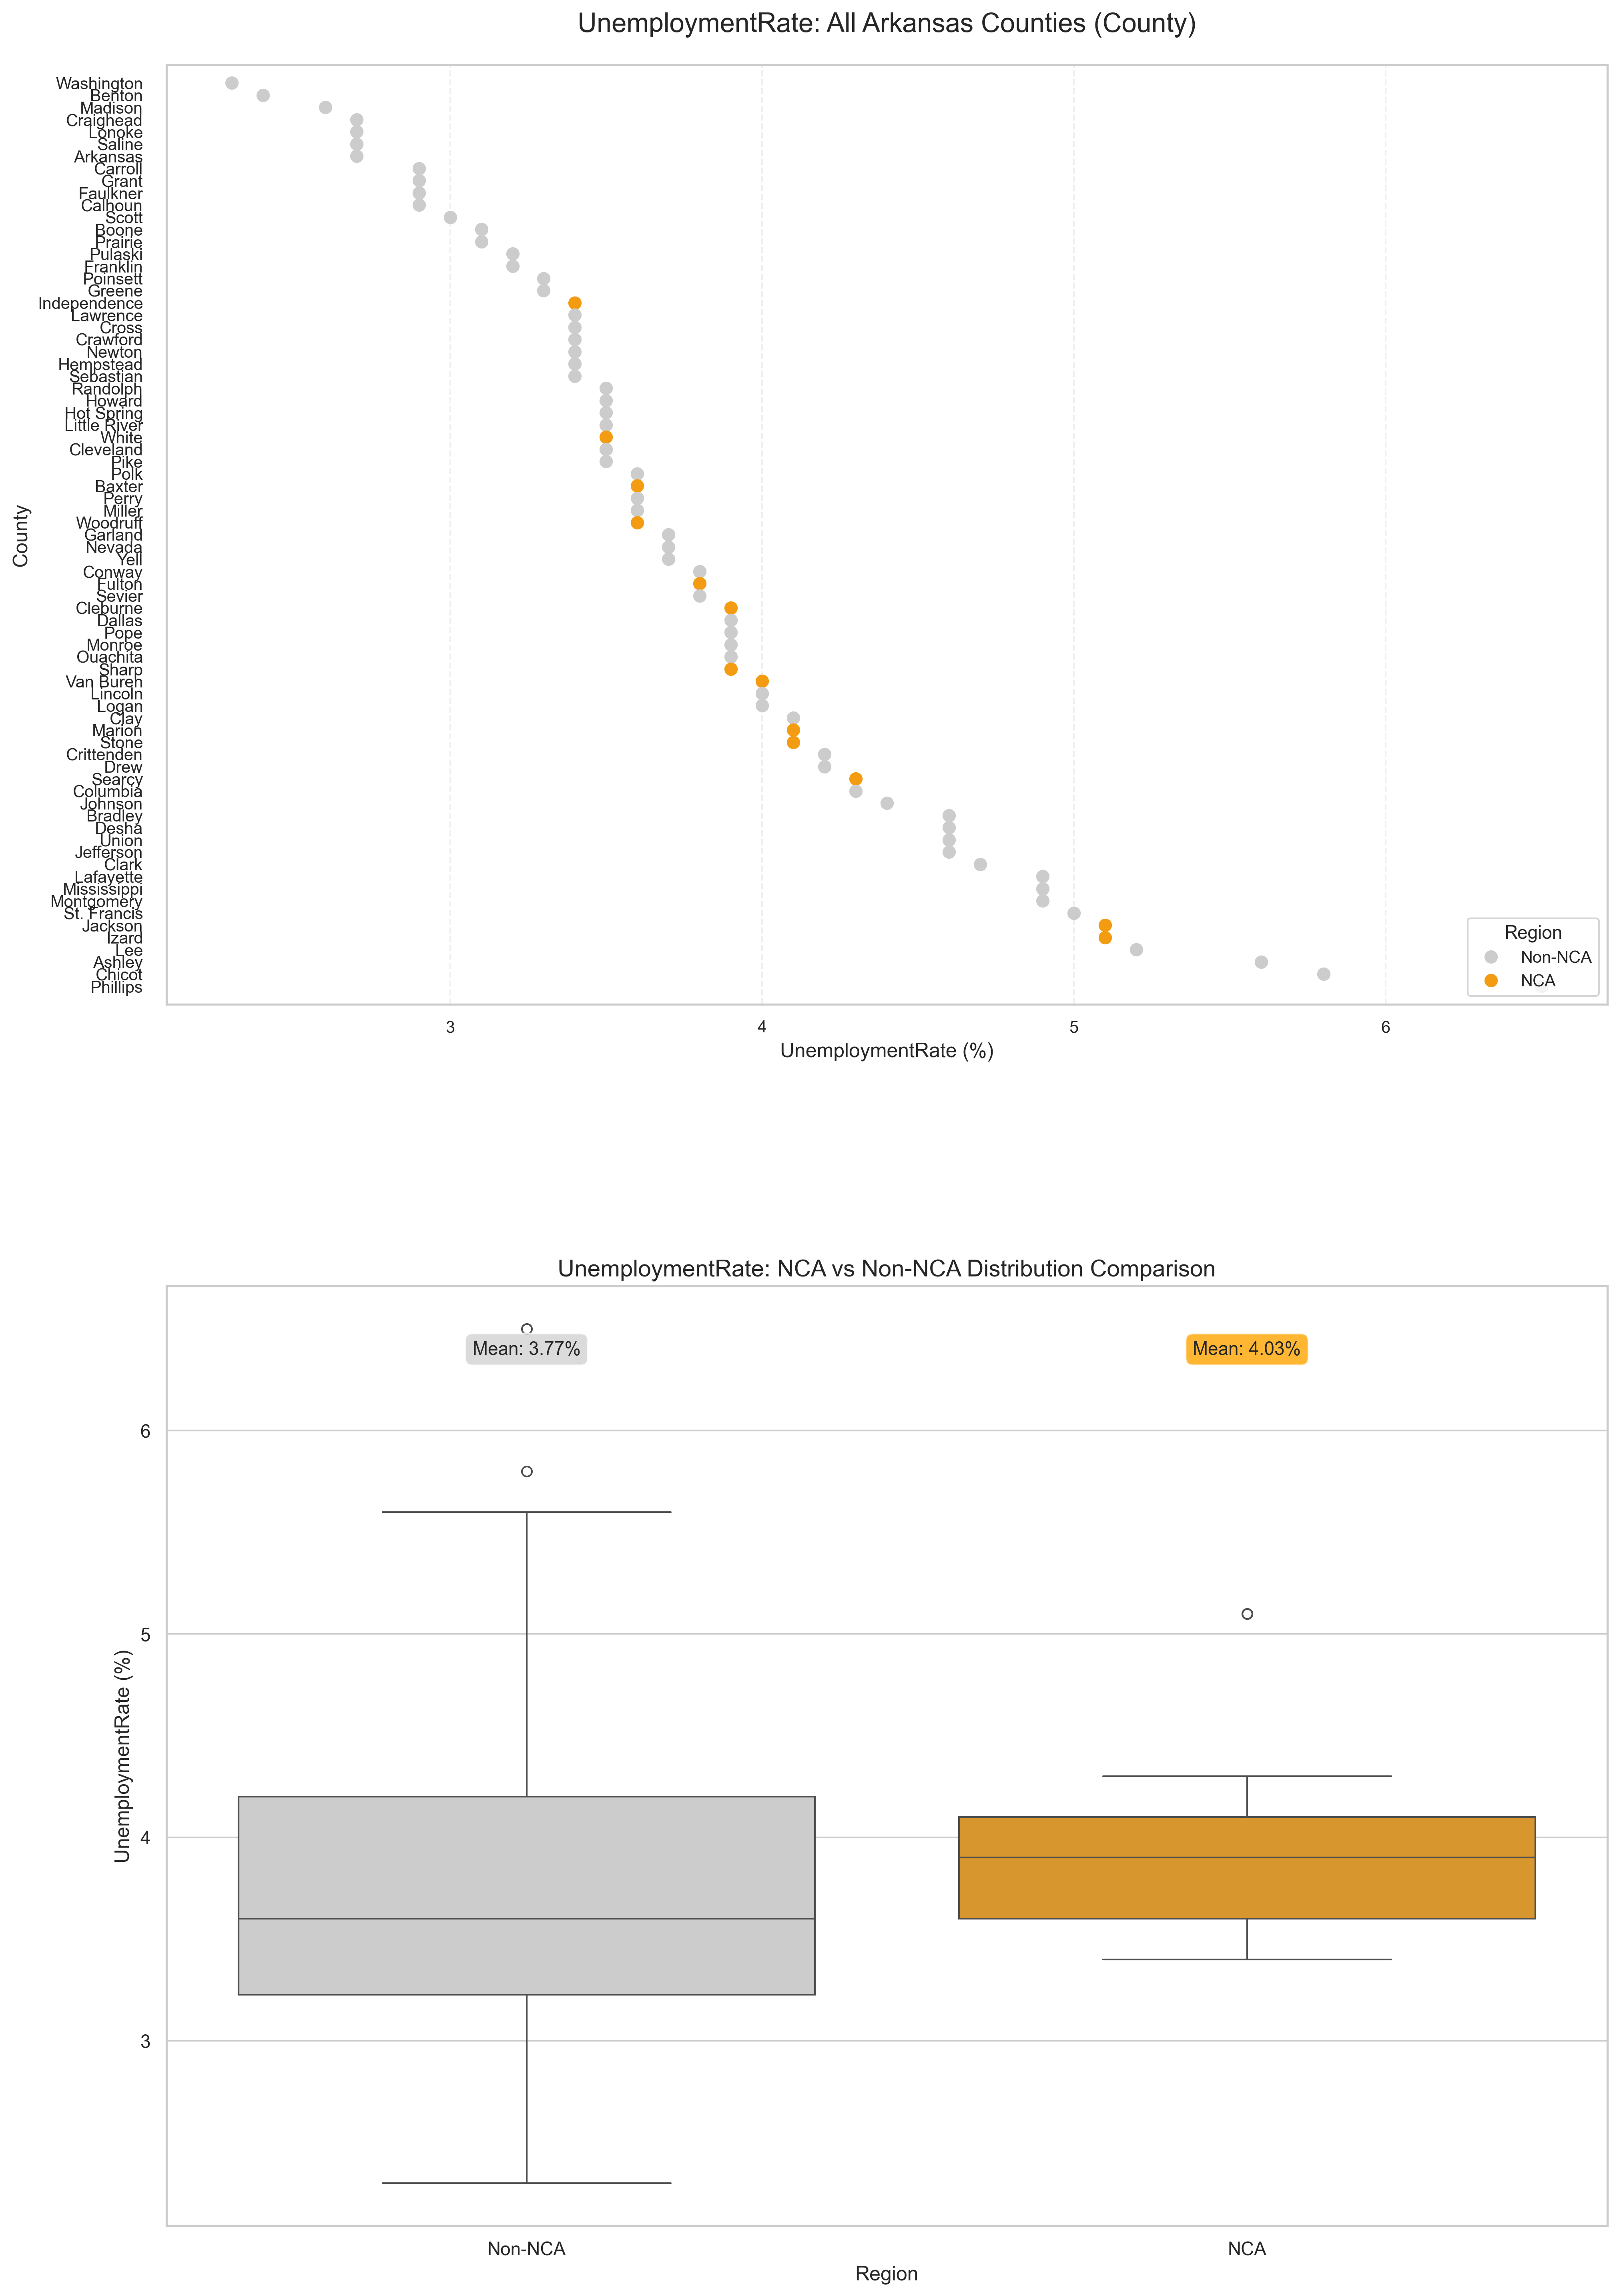
\includegraphics[width=0.95\textwidth]{Capstone_Project_Report/images/maps/nca_comparison_unemploymentrate.png}
\caption{Bivariate Comparison of Unemployment Rates: While the majority of NCA counties align with the state average in unemployment, a few exhibit elevated levels that may signal localized labor market challenges. This figure supports the case for further investigation into county-specific employment dynamics.}
\label{fig:appendix_unemployment}
\end{figure}



